%!TEX root = ../../super_main.tex

\section{Existing Solutions}
\label{sec:existing_solutions}

Some solutions that use data gathering have been investigated, of which some are intended to be used in the area of mental health. It seems that a lot of software has been designed to improve this area based on mobile sensor data gathering. We discuss four solutions which monitor subjects using smartphone sensors, and in some cases have these subjects fill out surveys. We here refer to subjects as people who use a data gathering systems for some purpose.

\subsection{Ilumivu mEMA}
\label{sub:ilumivu_mema}
In mental health care there exists a concept called Ecological Momentary Assessment (EMA) \parencite{shiffman2008ecological}, which is a way of making assessments of patients in the ecosystem where they normally exist. In traditional medical practice, the patient is acquainted with a doctor, and long term treatment consists of periodical appointments with a doctor. This particular pattern has disadvantages in psychological treatments where the treatment does not happen in the environment where the patient lives, but it happens in a doctor's or psychiatrist's office. EMA is a way of gathering information about patients, and possibly providing some sort of treatment or intervention in real-time. This type of system works well with mobile technologies, because they have a variety of sensors available.
\\\\
Ilumivu has developed a Mobile EMA (mEMA) application \parencite{lumivu}. A screenshot of the application can be seen in \figref{fig:ilumivu_screenshot}. This application provides researchers and companies, i.e. the customers, with a platform for real-time data gathering from test subjects going about their daily lives. The functionality in the purchasable core package includes questionnaires and the creation of these. It is also possible for the customers to add certain opt-ins, that can provide more information about the context for the answers of the questionnaires, such as mobile sensors, wearable sensors, and in-home sensors. The system is centered around the patient, and is generally meant for research purposes.

\begin{figure}[!htbp]
	\centering
	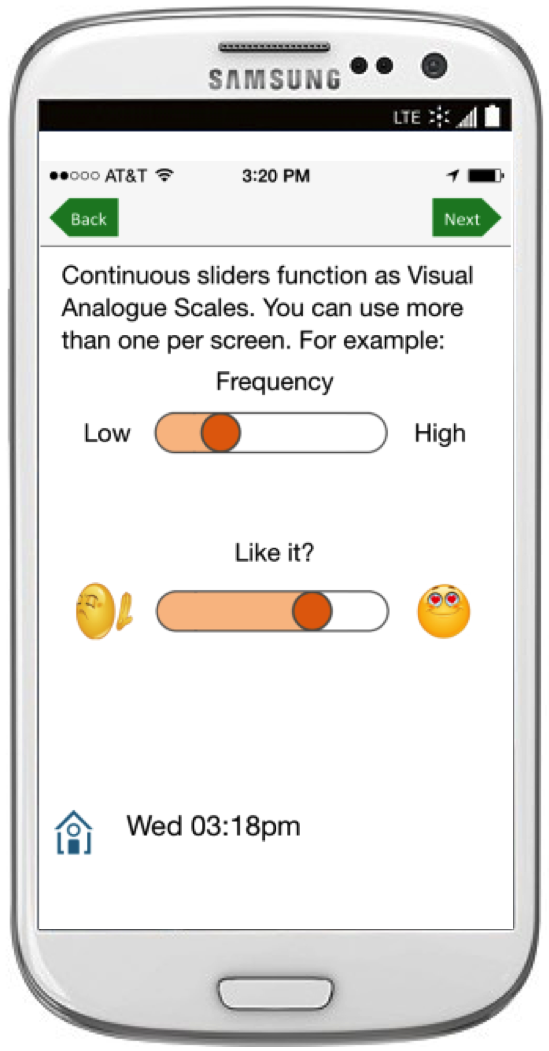
\includegraphics[height=0.5\textwidth]{graphic/existing_solutions/ilumivu.png}
	\caption[]{Screenshot of the Ilumivu application\parencite{lumivu}.}
	\label{fig:ilumivu_screenshot}
\end{figure}
\FloatBarrier

\subsection{AndWellness}
\label{sub:andwellness}
AndWellness \parencite{hicks2010andwellness} is another sensor monitoring/questionnaire focused system for Android phones. A screenshot of the application can be seen in \figref{fig:andwellness_screenshot}. AndWellness has some interesting ideas and principles on how to do this type of monitoring. This system has a concept of a campaign, which is the blueprint of a study, meaning it is the configuration of how sensor data is gathered and which questions their surveys should include. These configurations include how sensors should be monitored in terms of frequency and duration. It is also possible to configure how subjects are notified. AndWellness allows configuration of different triggers for questionnaires. These triggers can be set to be both temporal but also sensor activity based, meaning that both time and the activity and movement of the user can trigger sensor monitoring and notifications with surveys. This means that the customers using AndWellnes is able to customize their study in great detail, which is preferable as the purpose of the gathered data may vary. Lastly an idea to note is that this system has a concept of expiring surveys, meaning that the customer can configure for how long the subject may prolong a survey with a time window where the survey exists. These time windows allows customers to disallow metacognition, the process of reflecting about one's own thoughts.

\begin{figure}[!htbp]
	\centering
	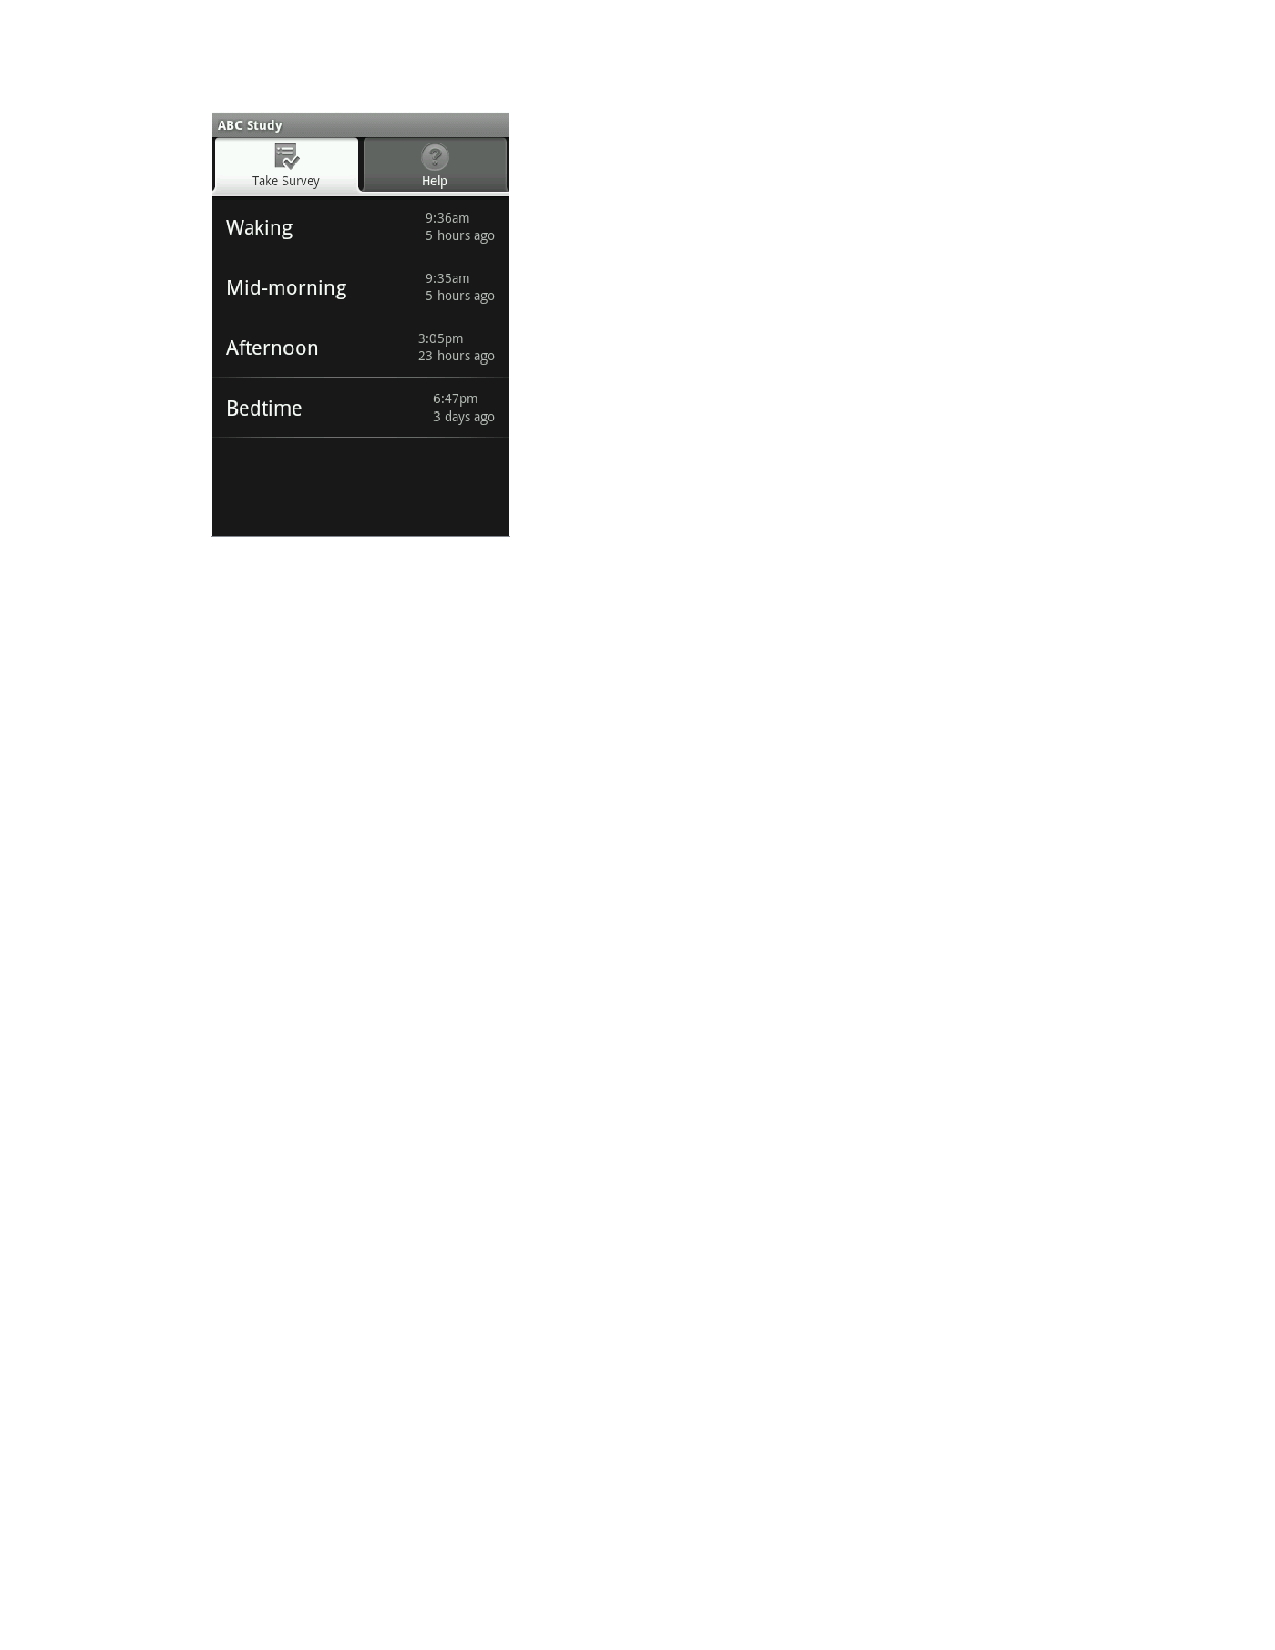
\includegraphics[height=0.5\textwidth]{graphic/existing_solutions/and_wellness.pdf}
	\caption[]{Screenshot of the AndWellness application\parencite{hicks2010andwellness}.}
	\label{fig:andwellness_screenshot}
\end{figure}
\FloatBarrier

The AndWellness system allows for full transparency, meaning that subjects have full access to the data they are gathering for the customers, to increase trustworthiness. Lastly AndWellness does not support raw sensor output logging, they derive some virtual sensors which they call Location- and Activity trace sensors. This is a potential flaw, because the data used to derive output cannot be converted back to raw sensor output and a mental health study might need data which is not included in the outputs of these predefined virtual sensors.
\\\\
Ilumivu and AndWellness both monitor and report sensor readings in real time, meaning that they are highly connectivity dependent. It is not clear what these systems do in cases where there are no network access, but they stream the data directly to a server in almost real time when the phone is connected to a network. This type of network communication is counter intuitive with general practices on battery and network management. Furthermore these systems do not yet include a larger ecosystem of devices. For instance, these systems do not consider wearable technologies such as smartwatches and smart bands. This excludes some potential sensor information which is usually not present in smartphones.

% + Principle of campaign. %
% + Sensor monitoring have configurable resolutions (our terms: measurement frequency, sample duration, sample frequency).
% + Have different triggers, temporal, contextual (sensor). 
% + Triggers can both be camgaign-wise and participant specific.
% + Prompts for surveys.
% + Surveys expire, configured by admins of campaign (answering window).
% + Users have full transparency of the data gathered
% - Pure realtime, battery drain, very network dependent.
% - Pure smartphone, no wearable technology.
% - Only two derived (software sensors), Location and Activity tracing.
%     - No raw sensor output
% Purple Robot
\subsection{Purple Robot}
\label{sub:purple_robot} 
Purple Robot \parencite{purple_robot} is an Android application originally developed to allow for easier or better integration for the PhoneGap\footnote{http://phonegap.com/} and Apache Cordova\footnote{https://cordova.apache.org/} applications with native functionality on the Android platform. The application, of which a screenshot can be seen in \figref{fig:purple_robot_screenshot}, allows other non-native applications to trigger status-bar notifications, application widgets, and full native dialogs. The application also allows other applications to access all the sensors on a device with an uniform interface. The communication for triggering and reading of the sensors is done using a locally running Hypertext Transfer Protocol server, that the Purple Robot application runs. This means that the Purple Robot application actually does not provide a lot of functionality for human activity recognition on its own, but allows other applications to have easy access to the integrated native functionality. This framework could be used to create access to native functionality, i.e. the sensors of an Android device, without having to build and maintain an Android application. Users could be asked to download and install Purple Robot instead. The framework supports delayed and encrypted uploads of collected data. However, when we tried out this application it seemed to be unstable, and would often crash. This might also be the case for other users, which might make them less willing to use the application.

\begin{figure}[!htbp]
	\centering
	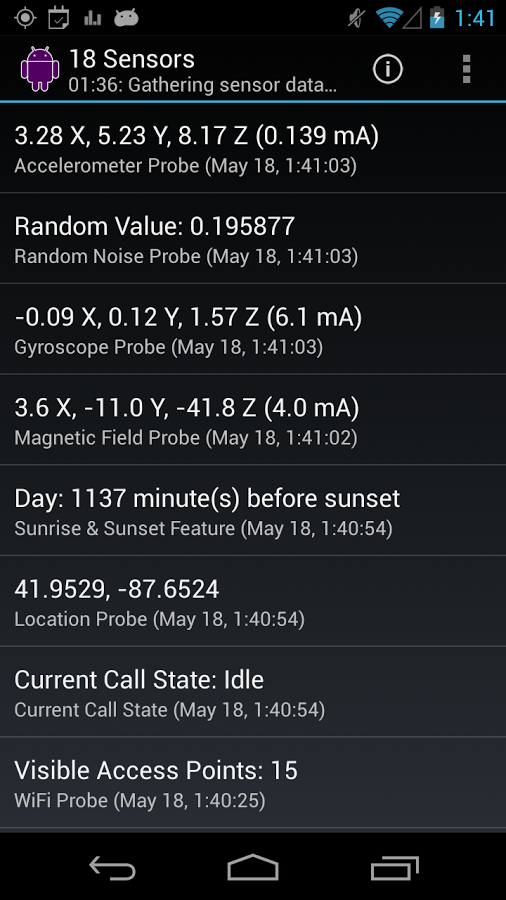
\includegraphics[height=0.5\textwidth]{graphic/existing_solutions/purple_robot.png}
	\caption[]{Screenshot of the Purple Robot application\parencite{purple_robot_google_play_store}.}
	\label{fig:purple_robot_screenshot}
\end{figure}
\FloatBarrier

\subsubsection{Using Third Party Applications}
It might already be a challenge for us to gain the trust of participants. We are handling sensitive information about their everyday activities and lives. Installing a third party application to handle this information, such as Purple Robot, could become a potential trust issue, and would require additional effort from the participants. As mentionend, we have installed the Purple Robot application on our devices and found the graphical user interface in the application to be unstable with seemingly random breakdowns. We have found this application and concept interesting, but we have found the application too unstable to be practical, and would instead like to handle the collection in another manner. 

\subsection{Sensor Data}
\label{sub:sensor_data}
Sensor Data is an iPhone application for gathering unlabeled data. A screenshot of this application can be seen in \figref{fig:sensor_data_screenshot}. The application can gather data from sensors that are available in iPhone devices, which is then made available through a web application programming interface. It is possible to store the sensor data in two different ways when using Sensor Data: Capture Mode and Streaming Mode. When using Capture Mode the data is stored directly into the flash memory of the iPhone, while using Streaming Mode will transfer the data to another device. The data is recorded and stored as comma separated values for easy integration into data analysis software.

\begin{figure}[!htbp]
	\centering
	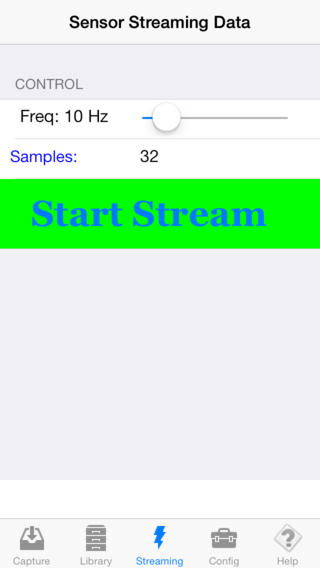
\includegraphics[height=0.5\textwidth]{graphic/existing_solutions/sensor_data}
	\caption[]{Screenshot of the Sensor Data application\parencite{sensor_data_app_itunes}.}
	\label{fig:sensor_data_screenshot}
\end{figure}
\FloatBarrier

There are a variety of existing solutions that make it possible to gather sensor data from a smartphone device, and even some that tie this sensor data with questionnaires about the mental health of the person being measured. There also exist solutions that are not meant to gather the data for themselves, but instead provide easy access to sensors for other applications. Most of the systems we have looked at do, according to their descriptions, not attempt to preserve battery when presenting the data to the users, which could be improved upon as we talk about in \secref{sec:general_strategies}. We have furthermore covered some interesting concepts that the other solutions use, such as Campaigns by AndWellness, which could be interesting to pursue in any further development. 